\documentclass{article}
\usepackage{graphicx} % Required for inserting images

\title{Final Report of Capstone project}

\bibliographystyle{plain}
\usepackage[hyphens,spaces]{url}

\begin{document}

\maketitle

\section{Team I\& Individual Accomplishments}  
Our team has managed to successfully complete the MVP as listed in our proposal. Here are some of the specific milestones we have achieved listed under each team member responsible for driving them: 

DebasishDas  – Core Application, Architecture, Documentation 
Worked on a simple web page what uses JavaScript library for ‘Google Maps Platform’ and ‘Bootstrap v5.0.2’ CSS. It allows a user to select a starting point and multiple destinations. Selecting a location comes with auto complete feature using ‘Google Maps API’. Then the user can get all the routes possible to traverse the destinations. ‘Heap Algorithm’ is used to find the permutation of the destinations [1]. Then each result of permutation was mapped on the distance matrix generated from ‘Google Maps API’. If the number of destinations is ‘n’, the time complexity is O(n!). n! number of routes would be generated.  I also tried Dijkstra and Floyd-Warshall’s algorithms, but found Heap algorithm more suitable to work on the distance matrix from ‘Google Maps API’. The generated routes are shown in the web page with detailed information (i.e., sequence of places, time and destinations). These routes can be filtered based on user’s choice link shortest distance, priority and priority. By default, the routes are showed as ascending order of total distance covered. Selecting a route will show it on Google Map. For simplicity and the technology stack that is familiar to all, I used Modular ECMAScript of JavaScript. However, it would be better to use React framework with NodeJS for an efficient development environment. 

Sai Nithish (2011242) – OpenstreetMap API, SingleSource-SingleDestination Problem, Architecture, Documentation, Report 

OpenStreetMap API:
I worked with the OpenStreetMap API, a project that offers free and editable map data, along with Application Programming Interfaces (APIs) for accessing and utilizing this data in applications. Several APIs are available for accessing OSM data and services. I initially used Leaflet and MapBox API to create a working version of the application. However, due to certain constraints and design choices, eventually we switched from OSM to the Google Maps API.

SingleSource-SingleDestination Problem:

While the DistanceMatrix service is useful for getting multiple route suggestions for more than one destination, it has limited functionality when dealing with a single source and single destination. This led to the need for a service that can fetch multiple routes in the case of SingleSource-SingleDestination scenarios. After exploring documentation and various solutions, I discovered the Direction service, which is also part of the Google Maps API. It accepts the origin, destination, driving mode, and a flag called provide Alternate Routes as part of the request, and in response, it provides geocoded waypoints. This response is then parsed, and the turns are calculated. Based on user preferences for sorting (e.g., total turns, left turns, right turns), multiple routes are displayed along with their estimated time of arrival (ETA) and distance. When the user selects a route and clicks on the "showMap" button, the corresponding route will be displayed on the map.

Technologies Used: 

	Web – HTML 5, CSS3, Bootstrap 5, JavaScript, GoogleMaps API(Direction Service).

	IDE: Visual Studio Code 1.79 
I worked on the JS files for placing a request to Maps API Direction service and then by parsing the response gathered the turns data for individual routes. This data is then sent over to a function which generates the html view which has the rendered turns data along with ETA and distance.

Sanad Mukadam (2032662) – UI Design, Architecture, Autocomplete, Authentication, UI Integration, Report Address Lookup I\& Autocomplete using Google Maps API: 
The Address lookup and autocomplete feature is an important aspect of our project. It is important for the user to be able to type in an address and be able to access autocompletion of addresses based on suggestions generated by the API used for lookup.

Technologies Used: 

	Web – HTML 5, CSS3, Bootstrap 5, JavaScript
	IDE: Visual Studio Code 1.79 
	Graphic Editor: Adobe Photoshop 
 
	Developed web page in HTML using CSS, JavaScript, and Bootstrap to allow user to enter Address and gives type-ahead-search functionality of Google map search field. The autocomplete service can match on full words and substrings, resolving place names, addresses,
	Embedded Google API to accomplish the task. 
	Developed webpage giving user two options  
	to enter address in one text box, 
	to enter address in first text box, based on which it will autofill other details like street address, city, state, zip code, country.  
	Uploaded webpage to GitHub repository. 

\begin{figure}
  \centering
  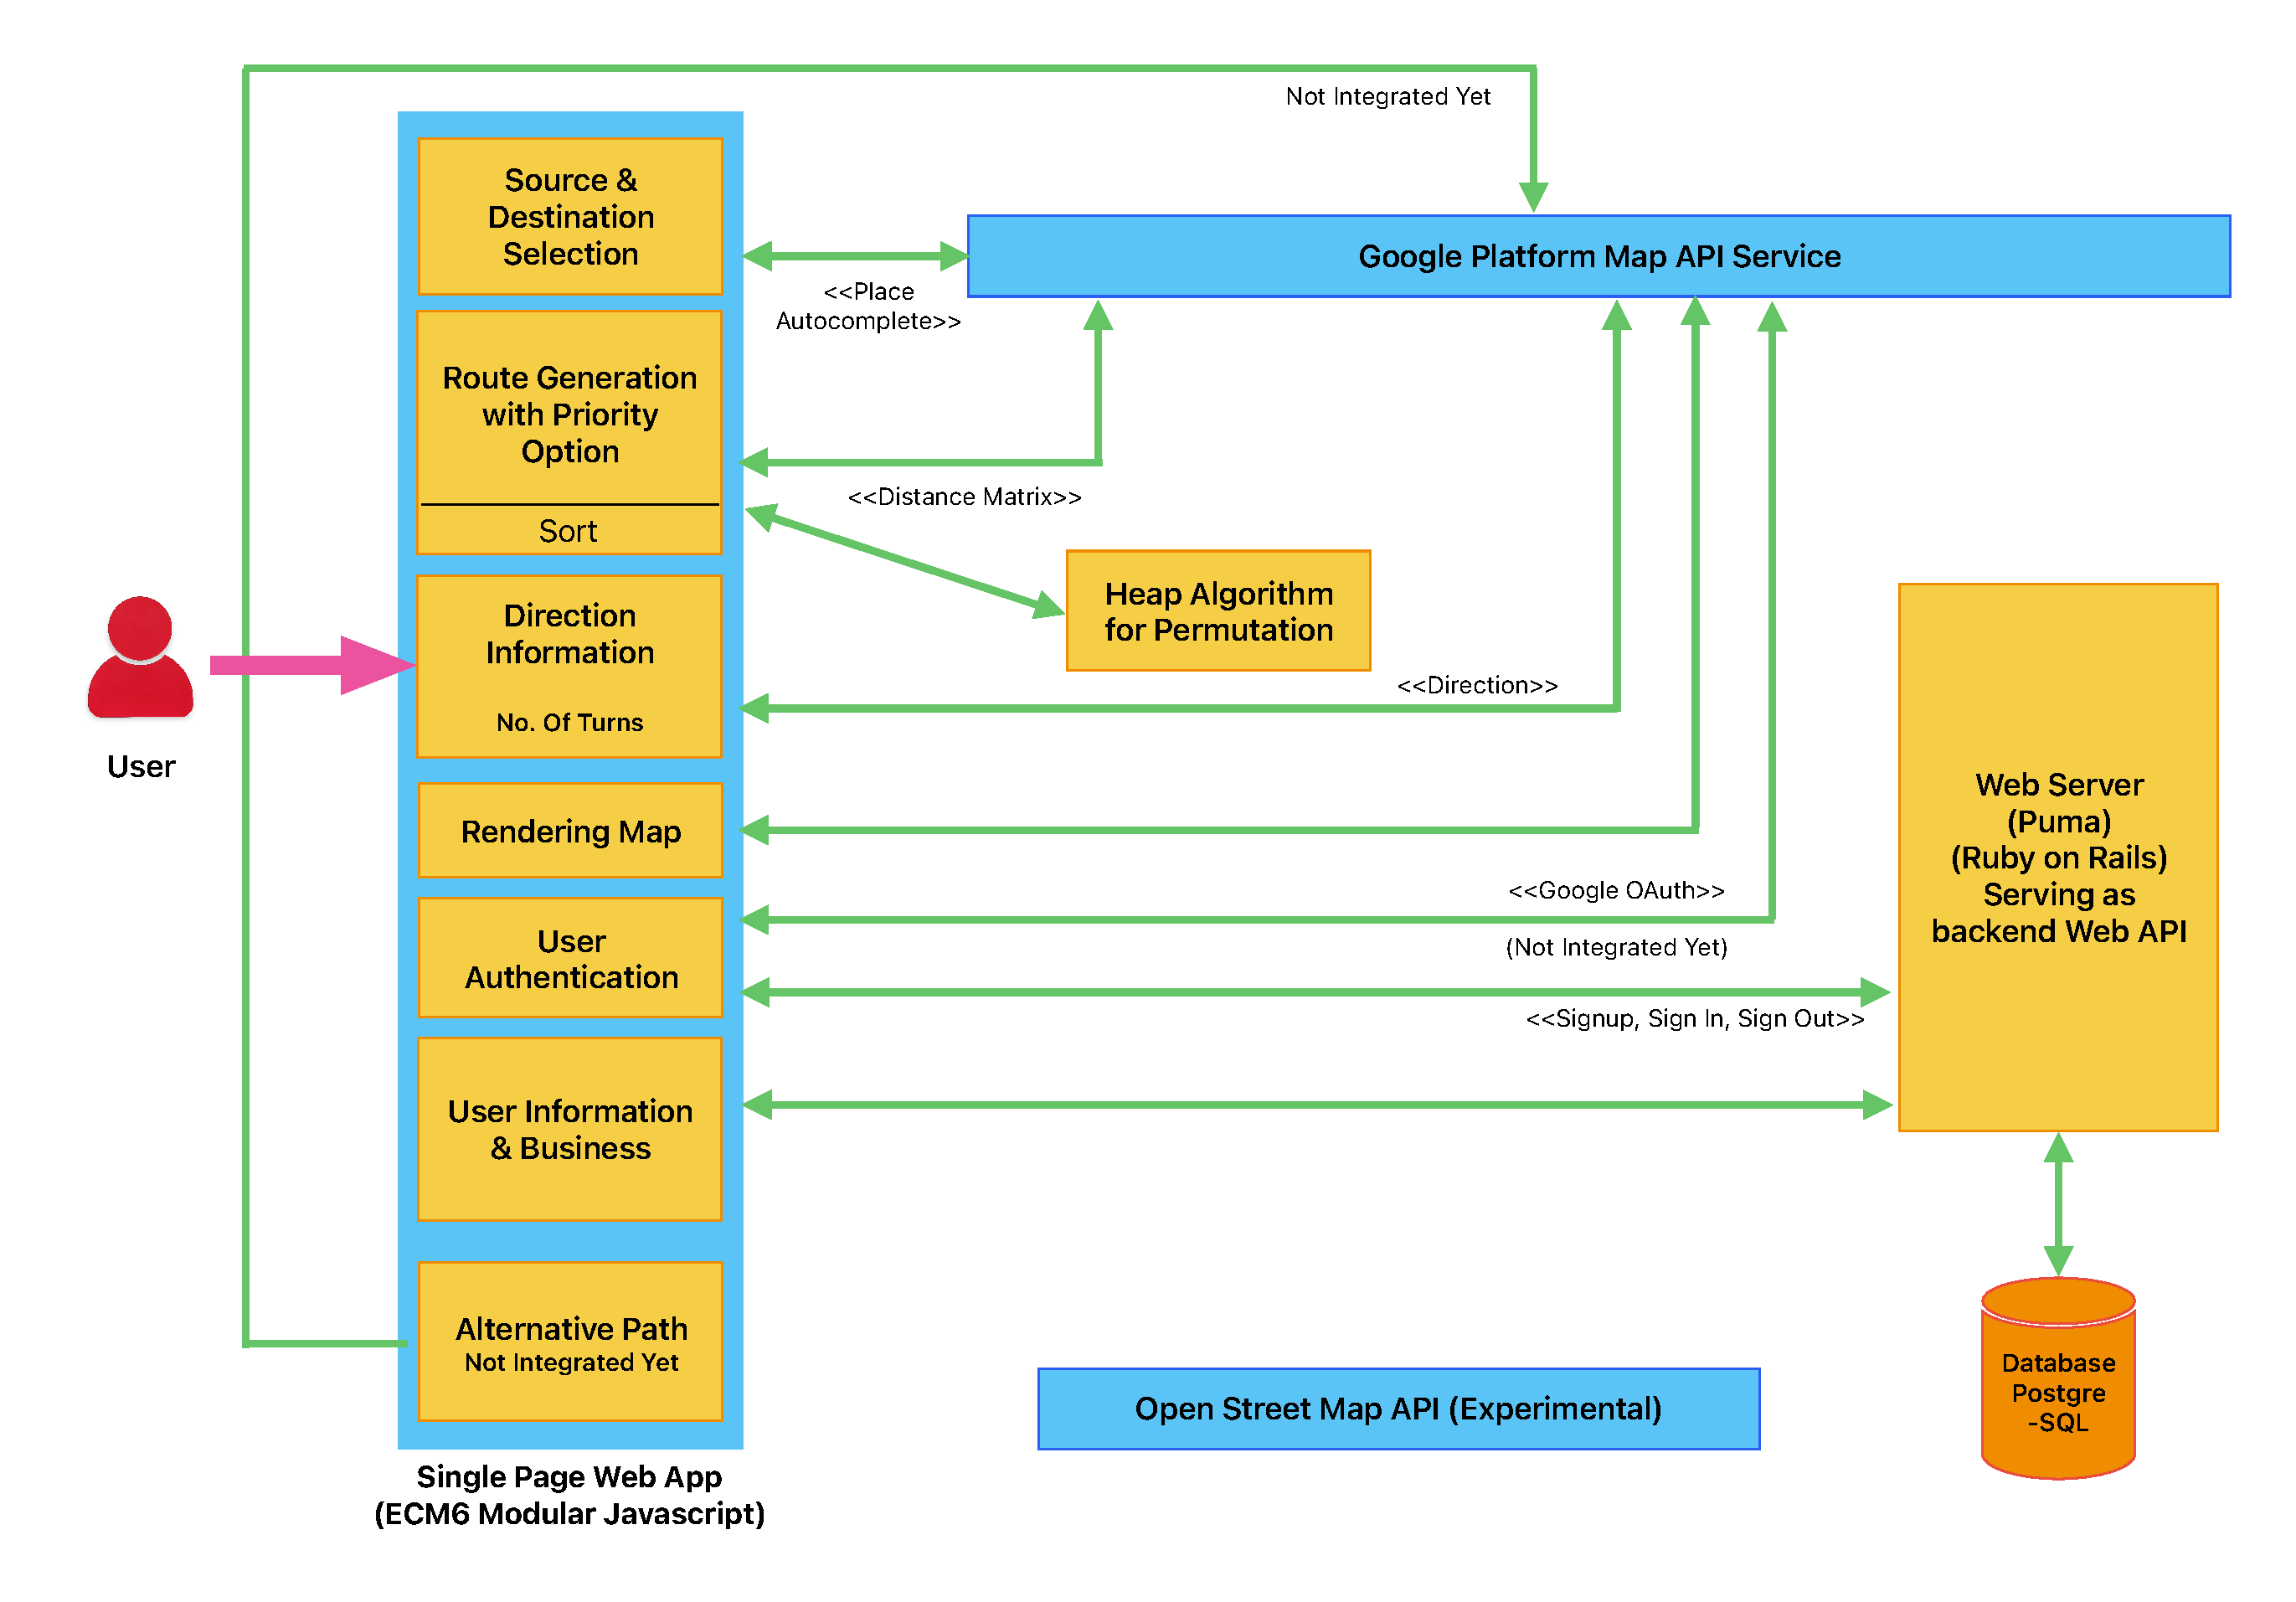
\includegraphics[width=1\textwidth]{NithishFinal/Architecture_v2.pdf}
  \caption{Architecture of Nav-Route}
  \label{fig:example}
\end{figure}


\begin{figure}
  \centering
  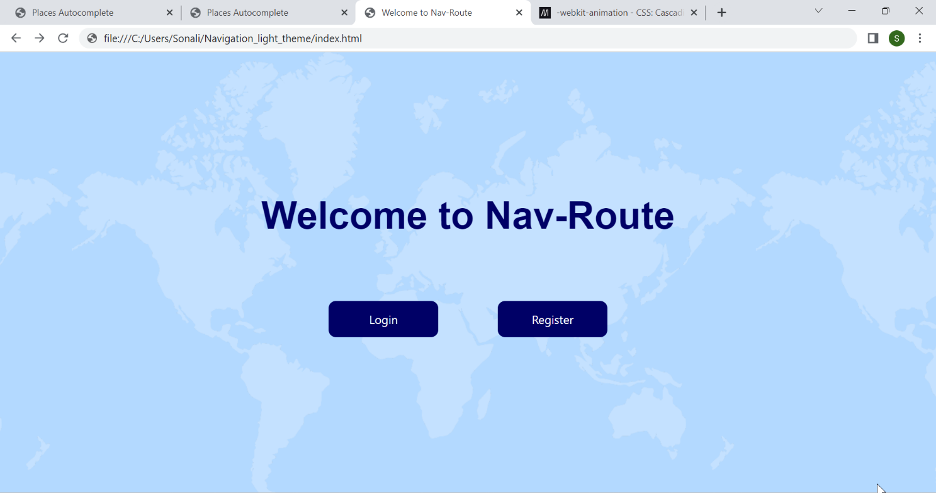
\includegraphics[width=1\textwidth]{NithishFinal/Picture5.png}
  \caption{Animated-background-theme }
  \label{fig:example}
\end{figure}

\begin{figure}
  \centering
  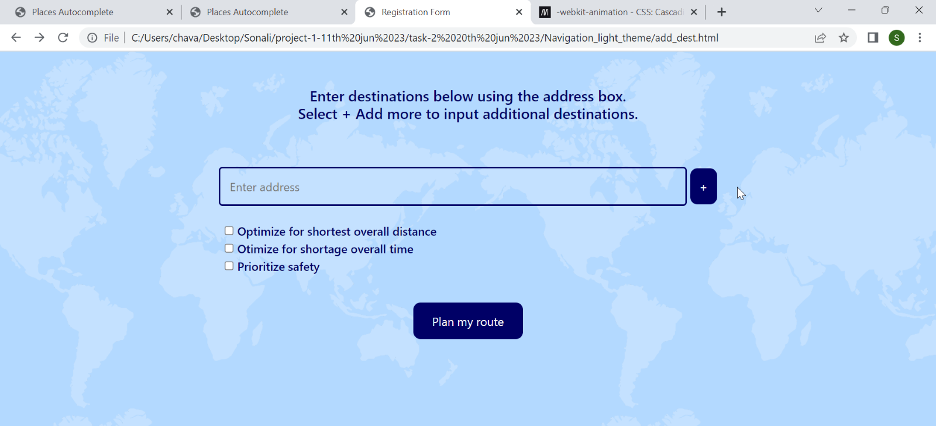
\includegraphics[width=1\textwidth]{NithishFinal/Picture6.png}
  \caption{Animated-background-theme }
  \label{fig:example}
\end{figure}

\begin{figure}
  \centering
  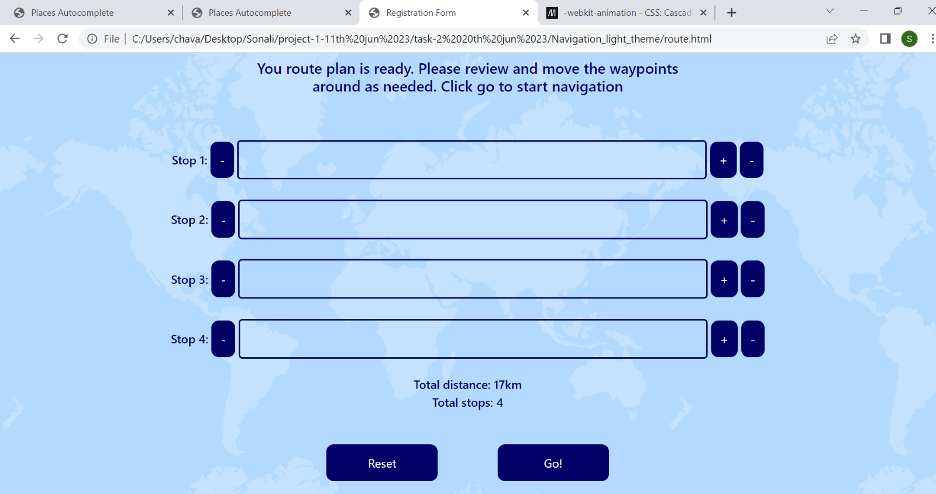
\includegraphics[width=1\textwidth]{NithishFinal/Picture7.png}
  \caption{Animated-background-theme }
  \label{fig:example}
\end{figure}

\begin{figure}
  \centering
  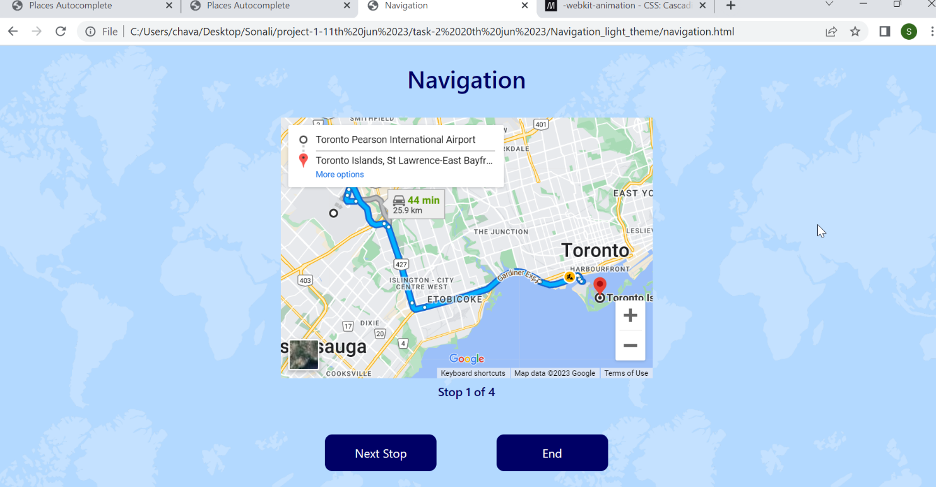
\includegraphics[width=1\textwidth]{NithishFinal/Picture8.png}
  \caption{Animated-background-theme }
  \label{fig:example}
\end{figure}

\begin{figure}
  \centering
  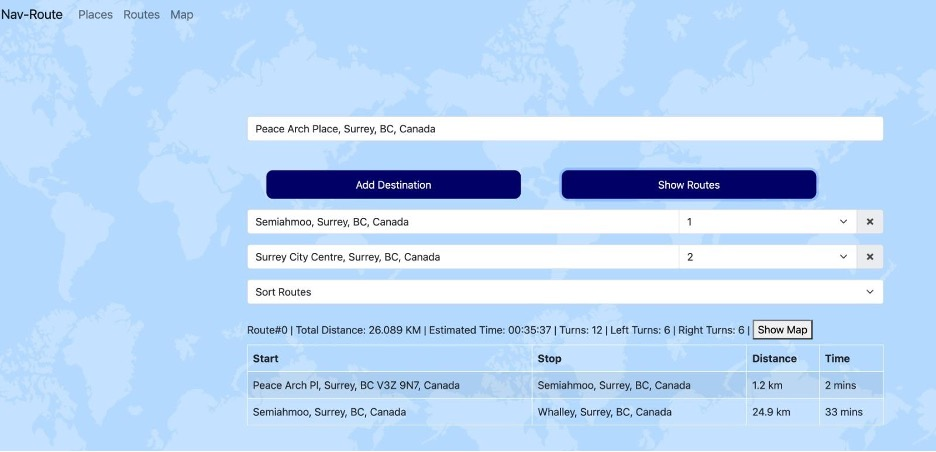
\includegraphics[width=1\textwidth]{NithishFinal/Picture9.jpg}
  \caption{Animated-background-theme }
  \label{fig:example}
\end{figure}

\begin{figure}
  \centering
  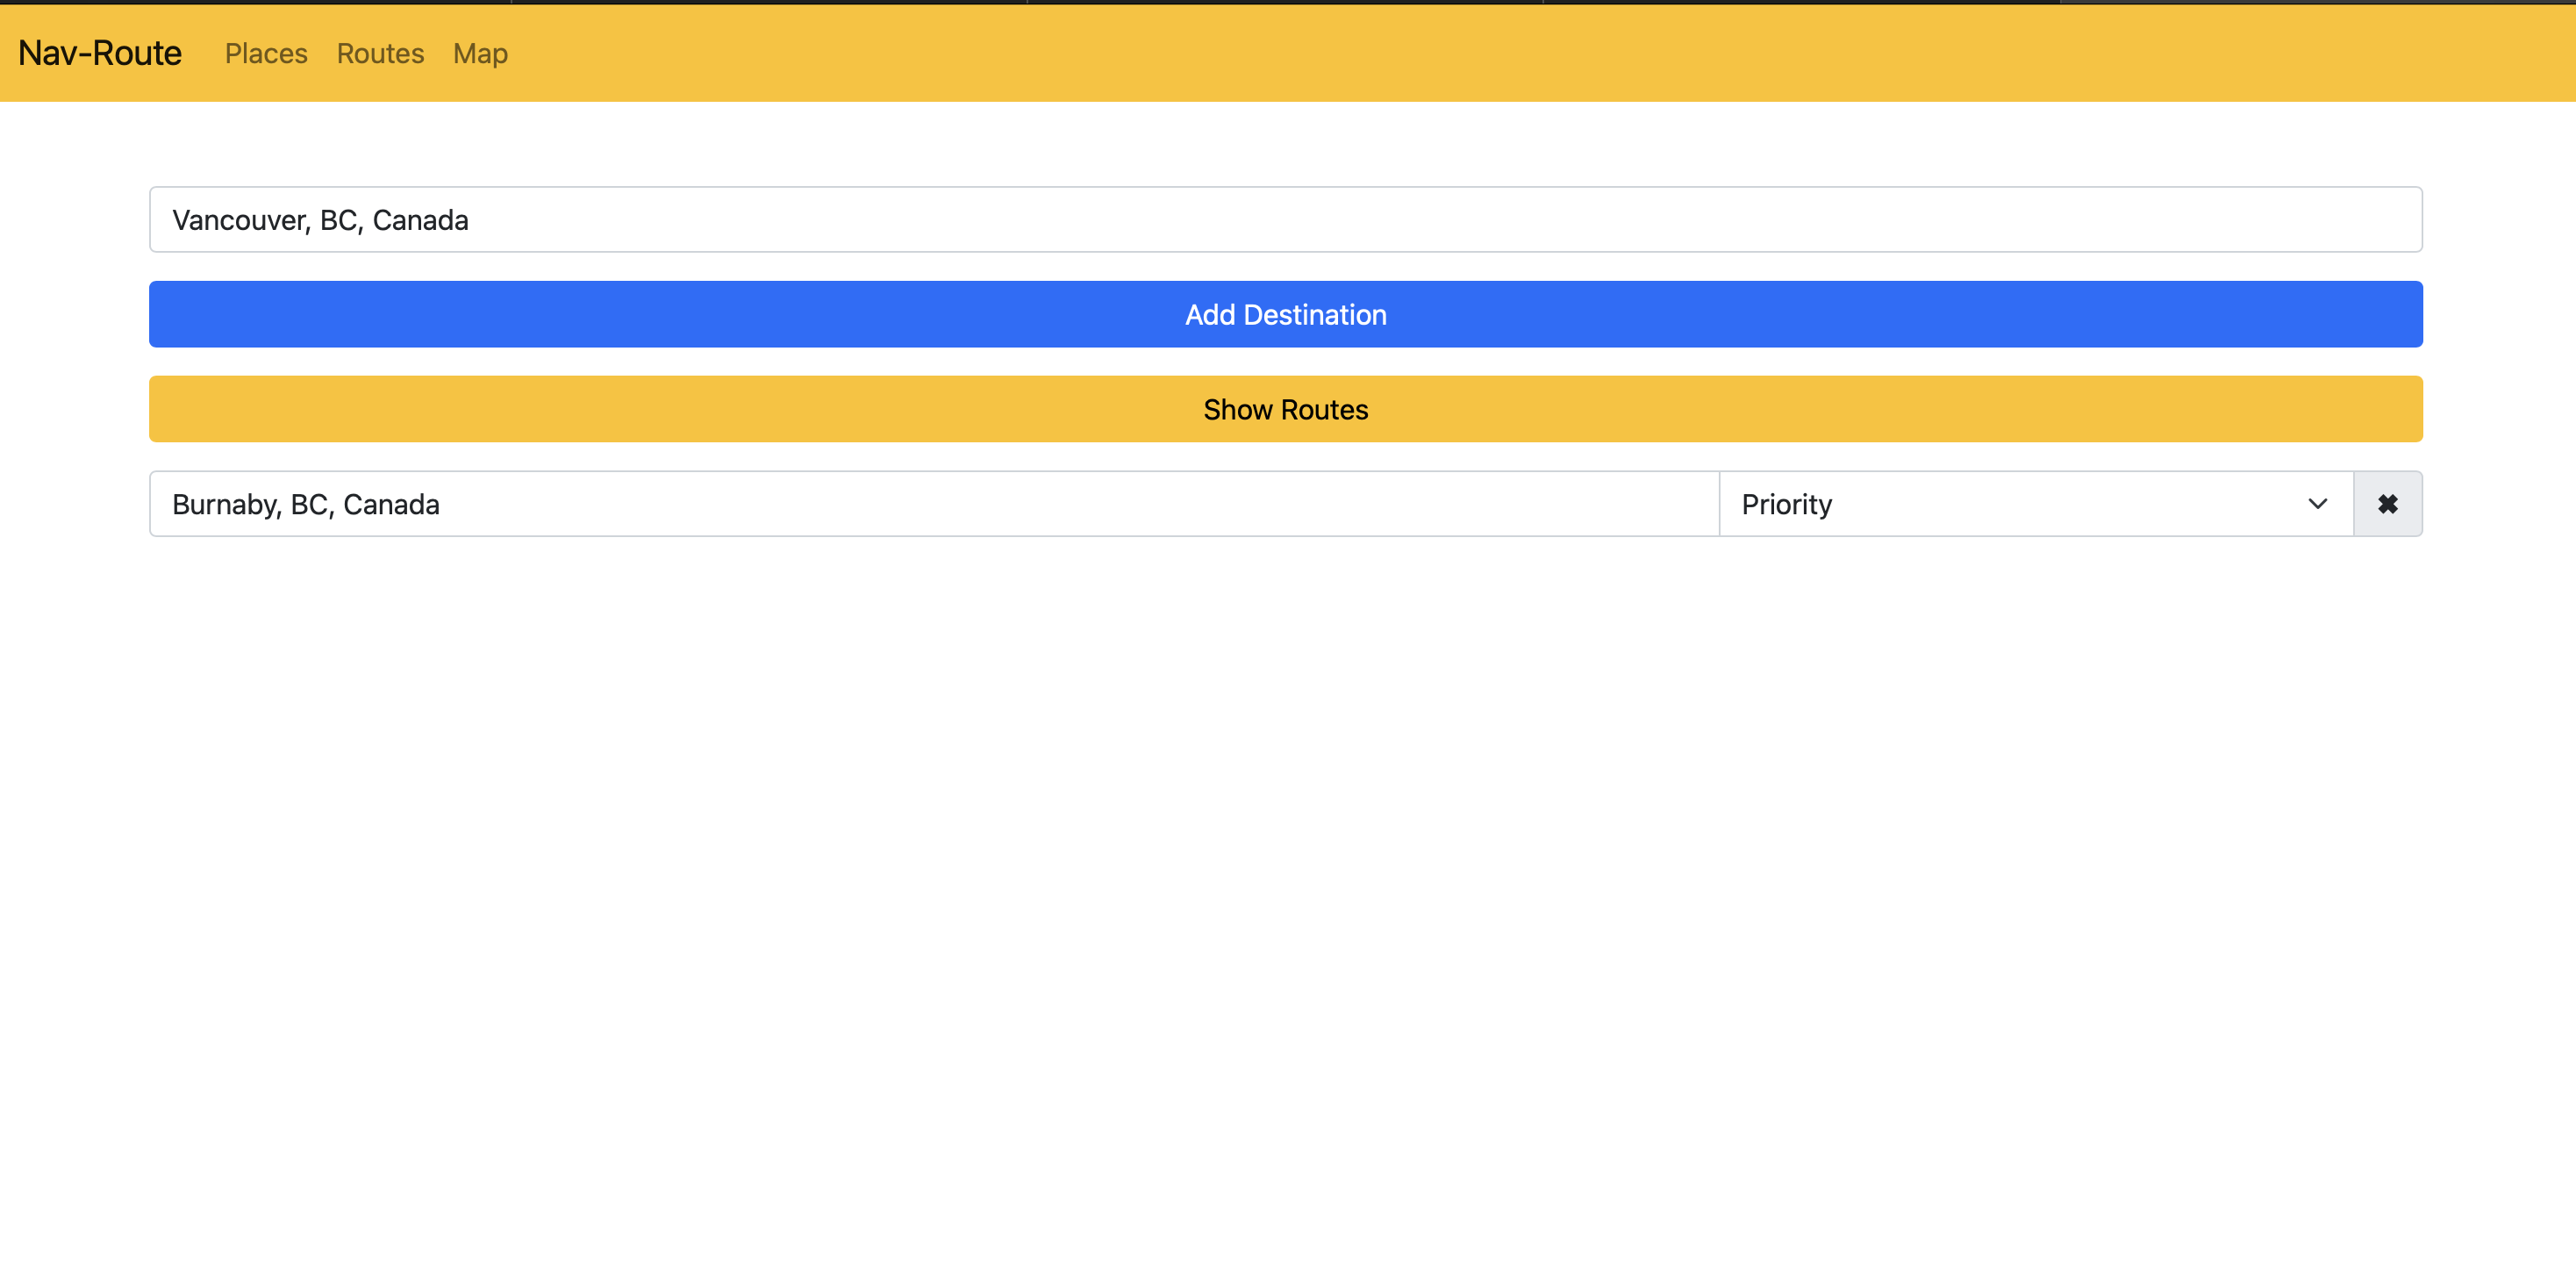
\includegraphics[width=1\textwidth]{NithishFinal/ARSS1.png}
  \caption{Alternative Route for Single Destination}
  \label{fig:example}
\end{figure}

\begin{figure}
  \centering
  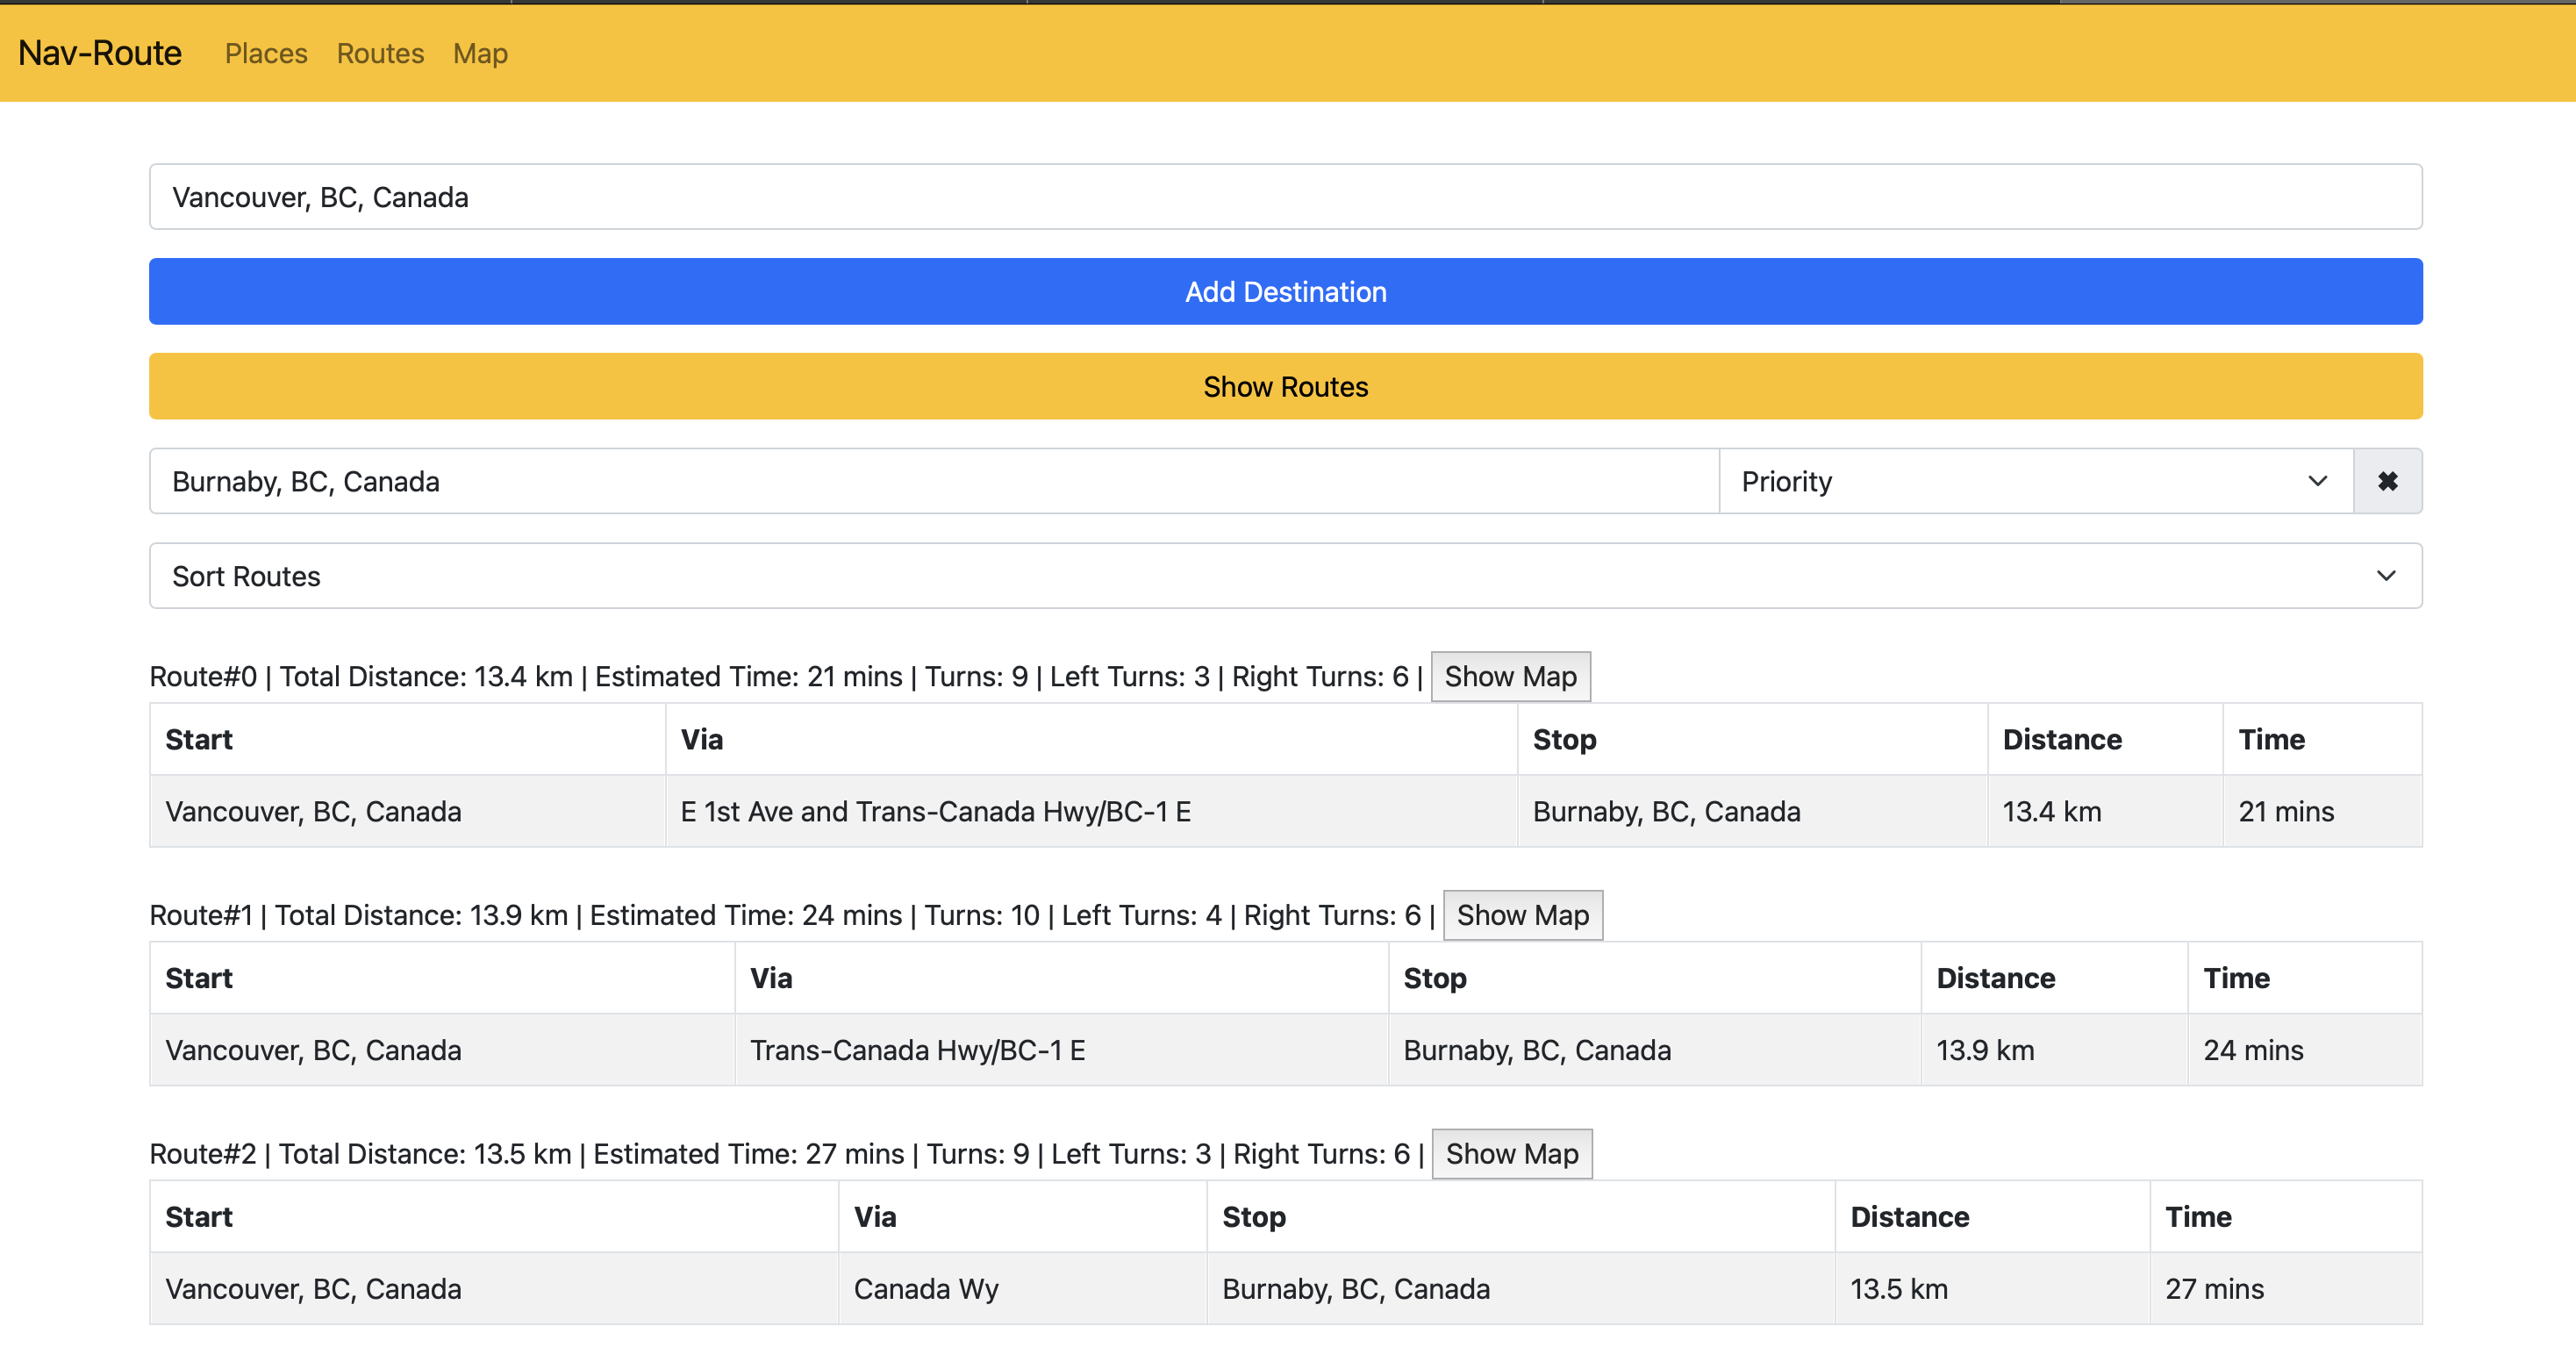
\includegraphics[width=1\textwidth]{NithishFinal/ARSS2.png}
  \caption{Multiple Routes}
  \label{fig:example}
\end{figure}

\begin{figure}
  \centering
  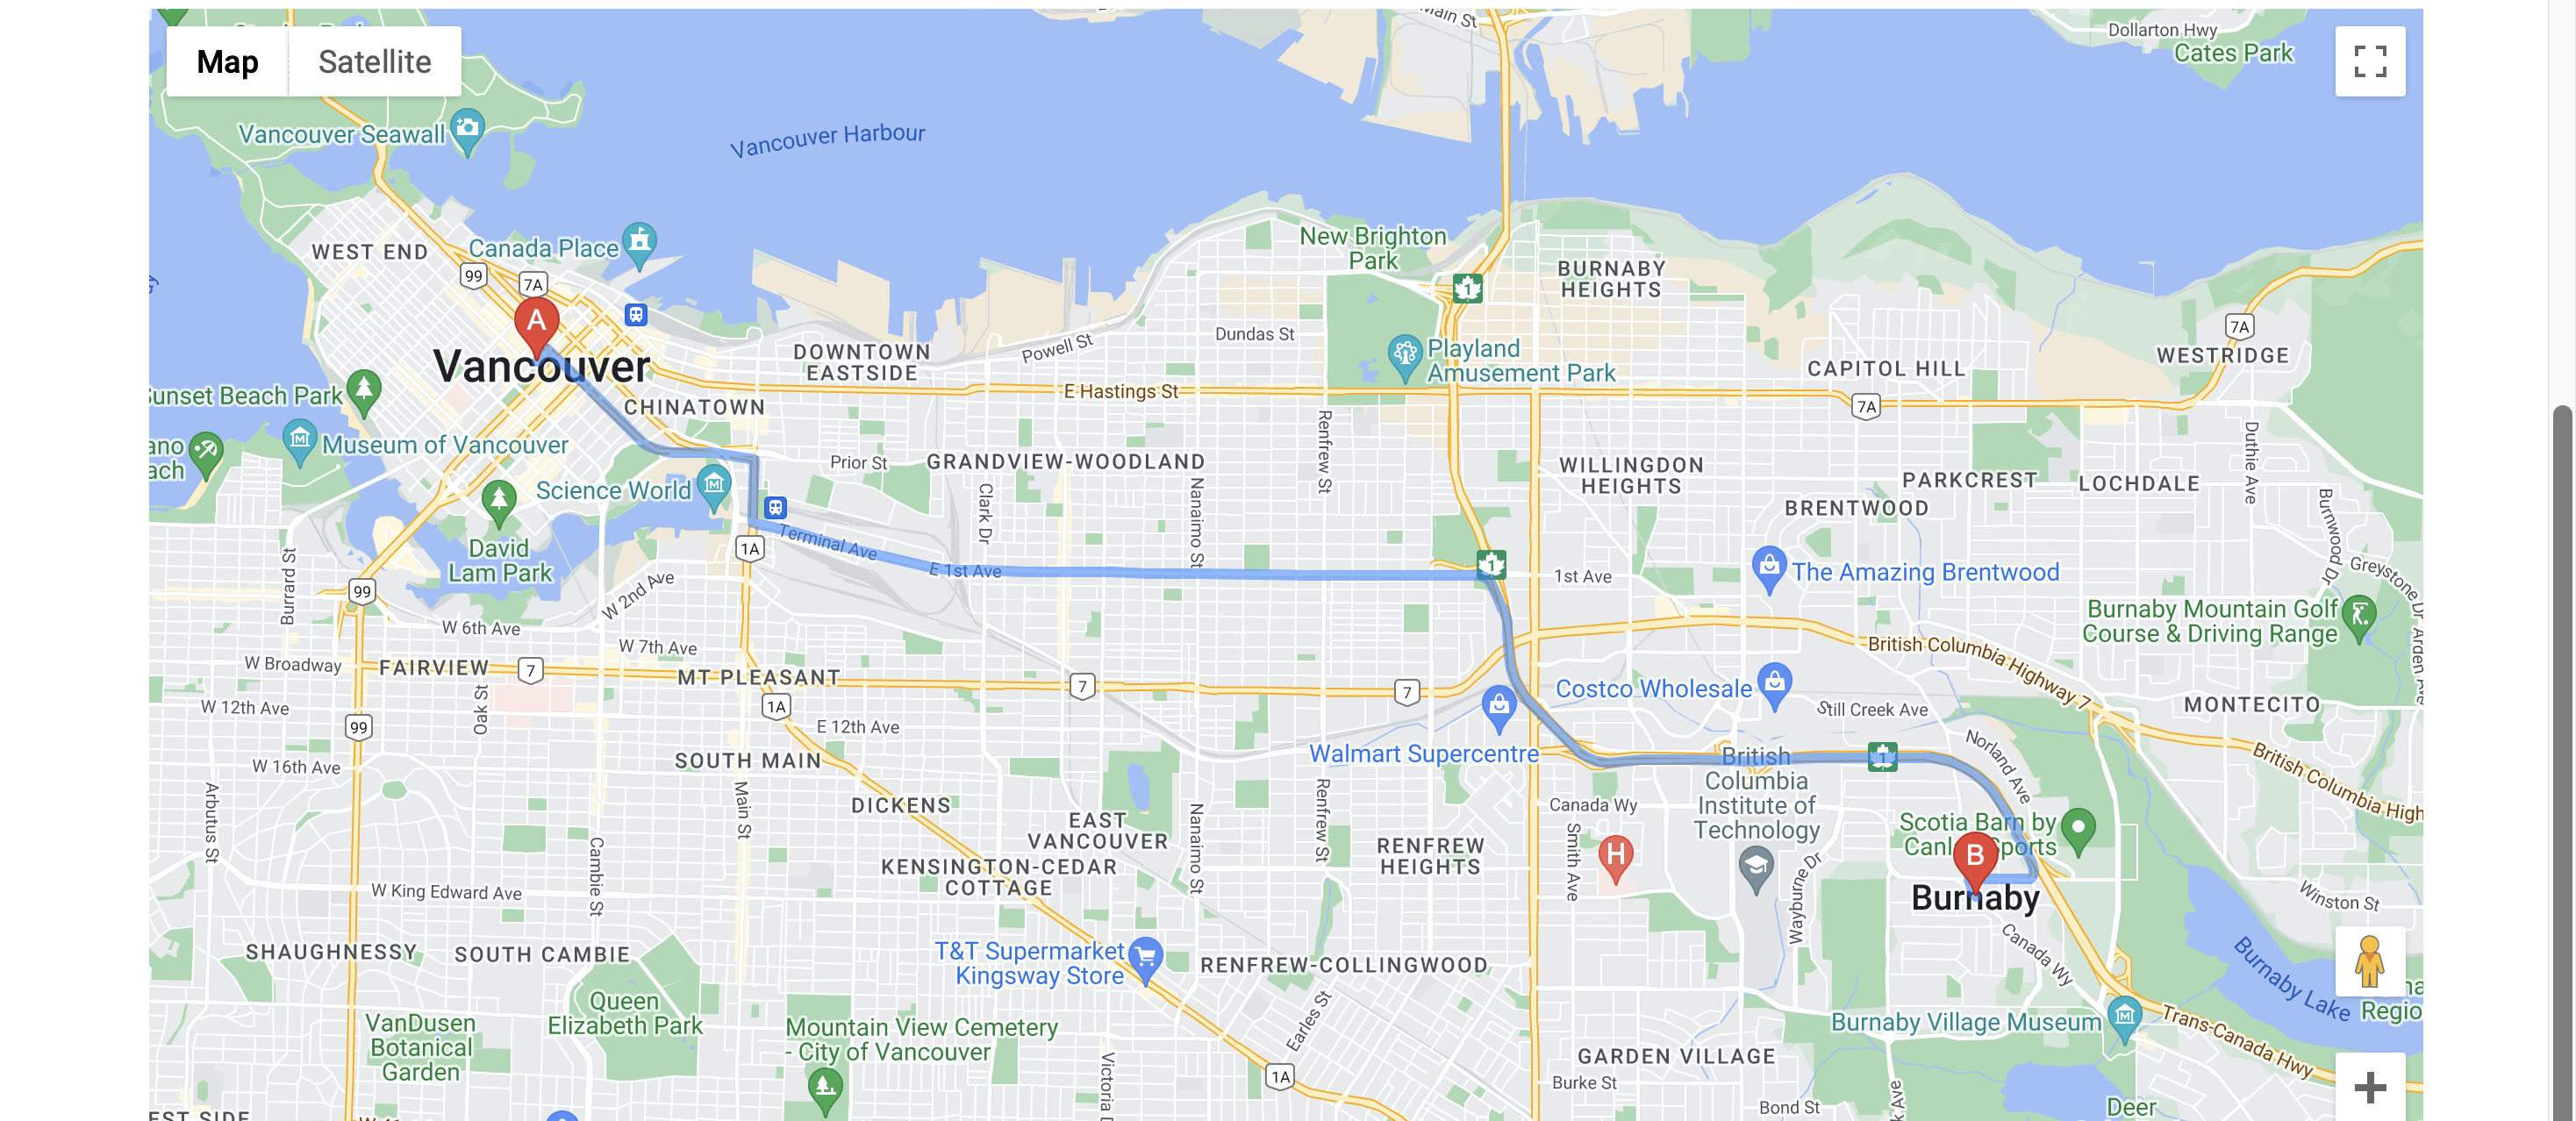
\includegraphics[width=1\textwidth]{NithishFinal/ARSS3.png}
  \caption{Display of Route on Map}
  \label{fig:example}
\end{figure}

In Figure \ref{fig:example}
\bibliography{final2.bib}

\end{document}